% Resultados
\section{Resultados}

% ── Slide 1: Benchmark ──
\begin{frame}
\frametitle{Benchmark econométrico — una referencia exigente}
\small
Con sólo 4 variables demográficas, los modelos lineales fijan una barra alta:

\vspace{0.3cm}
\centering
\scriptsize
\begin{tabular}{lrrrr}
\toprule
Modelo & Accuracy & AUC-ROC & F1 & CV AUC (5-fold) \\
\midrule
MCO (LPM) & 0.6611 & 0.7033 & 0.5823 & — \\
Probit     & 0.6611 & 0.7027 & 0.5817 & 0.6648 \\
\midrule
Random Forest     & 0.6397 & 0.6600 & 0.5689 & 0.6316 \\
Gradient Boosting & 0.6373 & 0.6947 & 0.5511 & 0.6667 \\
\textbf{GBM Tuneado} & \textbf{0.6573} & \textbf{0.6959} & \textbf{0.5891} & \textbf{0.6714} \\
\bottomrule
\end{tabular}

\vspace{0.3cm}
\flushleft
\scriptsize
\textbf{Hallazgo}: con hiperparámetros por defecto, el ML \textit{no} supera al benchmark.\\
El GBM tuneado apenas gana en CV5: $+0.007$ sobre Probit, $+0.005$ sobre AUC de prueba.\\
El benchmark no es formalidad; es una \textbf{restricción activa}.
\end{frame}

% ── Slide 2: Por qué el ML no gana por defecto ──
\begin{frame}
\frametitle{¿Por qué el ML no supera al benchmark por defecto?}
\begin{columns}[T]
\column{0.55\textwidth}
\centering
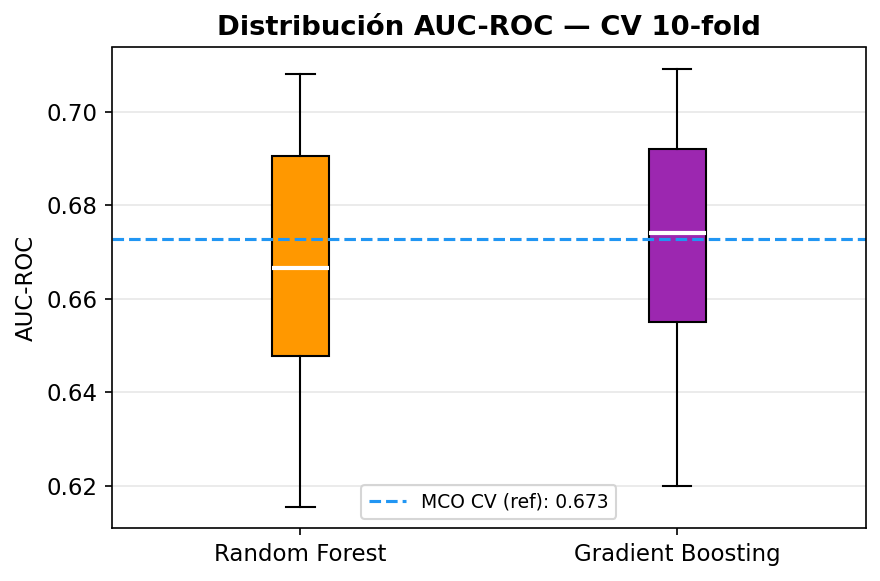
\includegraphics[width=\textwidth]{../figures/cv_10fold_boxplot.png}
\scriptsize CV-10 — solapamiento sustancial entre modelos

\column{0.42\textwidth}
\small
\textbf{Interpretación}:
\begin{itemize}
    \item Relación aproximadamente aditiva en 4 variables $\Rightarrow$ MCO minimiza sesgo.
    \item ML sin regularización paga varianza sin ganancia de sesgo.
    \item Las cajas de CV-10 se solapan: diferencias no robustas.
    \item El CV5 AUC del GBM tuneado (0.671) apenas supera al Probit (0.665).
\end{itemize}
\vspace{0.2cm}
\textit{La ganancia real vendrá de ampliar el feature set.}
\end{columns}
\end{frame}

% ── Slide 3: Tuning GBM (4-var) ──
\begin{frame}
\frametitle{Búsqueda de hiperparámetros sobre 4 variables — 300 evaluaciones}
\small
\textbf{Estrategia}: \texttt{RandomizedSearchCV}, 60 combinaciones × 5 folds estratificados.

\vspace{0.2cm}
\begin{columns}[T]
\column{0.42\textwidth}
\centering
\footnotesize
\begin{tabular}{lr}
\toprule
Hiperparámetro & Valor óptimo \\
\midrule
\texttt{n\_estimators} & 157 \\
\texttt{max\_depth} & 2 \\
\texttt{learning\_rate} & 0.042 \\
\texttt{subsample} & 0.972 \\
\texttt{min\_samples\_leaf} & 26 \\
\texttt{max\_features} & \texttt{log2} \\
\bottomrule
\end{tabular}

\column{0.55\textwidth}
\small
\textbf{Patrón interpretable}:\\[0.2cm]
Árboles muy superficiales (\texttt{depth=2}) + tasa baja + submuestra alta = \textbf{regularización agresiva}.

El ML gana no por mayor complejidad, sino por mejor control del compromiso \textbf{sesgo-varianza}.

\vspace{0.2cm}
\textit{Pero la ganancia sobre el benchmark es marginal con sólo 4 variables.}
\end{columns}
\end{frame}

% ── Slide 4: Modelo ampliado — resultados ──
\begin{frame}
\frametitle{Modelo ampliado — 16 variables, 7 grupos teóricos}
\small
\textbf{Muestra efectiva}: $n = 3\,401$ (eliminación por lista; 11.2\% de nulos en \texttt{regimen\_salud}).

\vspace{0.25cm}
\centering
\scriptsize
\begin{tabular}{lrrrr}
\toprule
Modelo (16 feat.) & $n$ & Accuracy & AUC-ROC & CV5 AUC \\
\midrule
Random Forest          & 3\,401 & 0.6397 & 0.6519 & $0.677 \pm 0.018$ \\
Gradient Boosting      & 3\,401 & 0.6490 & 0.6949 & $0.699 \pm 0.019$ \\
GBM Tuneado (16 vars)  & 3\,401 & 0.6505 & 0.6990 & $0.704 \pm 0.021$ \\
\textbf{RF Tuneado (16 vars)}   & \textbf{3\,401} & \textbf{0.6667} & \textbf{0.6995} & $\mathbf{0.703 \pm 0.007}$ \\
\midrule
\textit{Ref.: Probit (4 feat.)} & \textit{3\,980} & — & \textit{0.7027} & \textit{0.665} \\
\bottomrule
\end{tabular}

\vspace{0.3cm}
\flushleft
\scriptsize
\textbf{Lectura clave}: el CV5 AUC del RF Tuneado (0.703) supera al benchmark Probit (0.665) en \textbf{+0.038} y al GBM tuneado (4 vars) en \textbf{+0.032}. La varianza del RF ($\pm 0.007$) es \textbf{tres veces menor} que la del GBM tuneado ($\pm 0.021$), confirmando su estabilidad de generalización.
\end{frame}

% ── Slide 5: ¿Por qué RF? Justificación ──
\begin{frame}
\frametitle{Selección del modelo — ¿por qué RF Tuneado?}
\small
\textbf{Criterio}: menor varianza de CV5 + brecha \textit{train-test} controlada + máximo CV5 AUC.

\vspace{0.25cm}
\begin{columns}[T]
\column{0.48\textwidth}
\centering
\textbf{Hiperparámetros (RF regularizado):}\\[0.2cm]
\footnotesize
\begin{tabular}{lr}
\toprule
Parámetro & Valor \\
\midrule
\texttt{n\_estimators} & 400 \\
\texttt{max\_depth} & 15 \\
\texttt{max\_features} & 0.30 \\
\texttt{min\_samples\_leaf} & 25 \\
\texttt{min\_samples\_split} & 10 \\
\texttt{bootstrap} & True \\
\bottomrule
\end{tabular}

\column{0.50\textwidth}
\small
\textbf{Diagnóstico de ajuste}:\\[0.1cm]
\begin{itemize}
    \item AUC train = 0.760, AUC test = 0.700
    \item Brecha = \textbf{0.060} (antes 0.094)
    \item Curva de aprendizaje \textbf{estable}: no memorización
    \item CV5 $\pm 0.007$: la menor de todos los modelos
\end{itemize}
\vspace{0.1cm}
\textit{Regularización explícita: profundidad + hojas mínimas + bagging.}
\end{columns}
\end{frame}

% ── Slide 6: Curva de aprendizaje RF ──
\begin{frame}
\frametitle{Curva de aprendizaje — RF Tuneado (16 variables)}
\centering
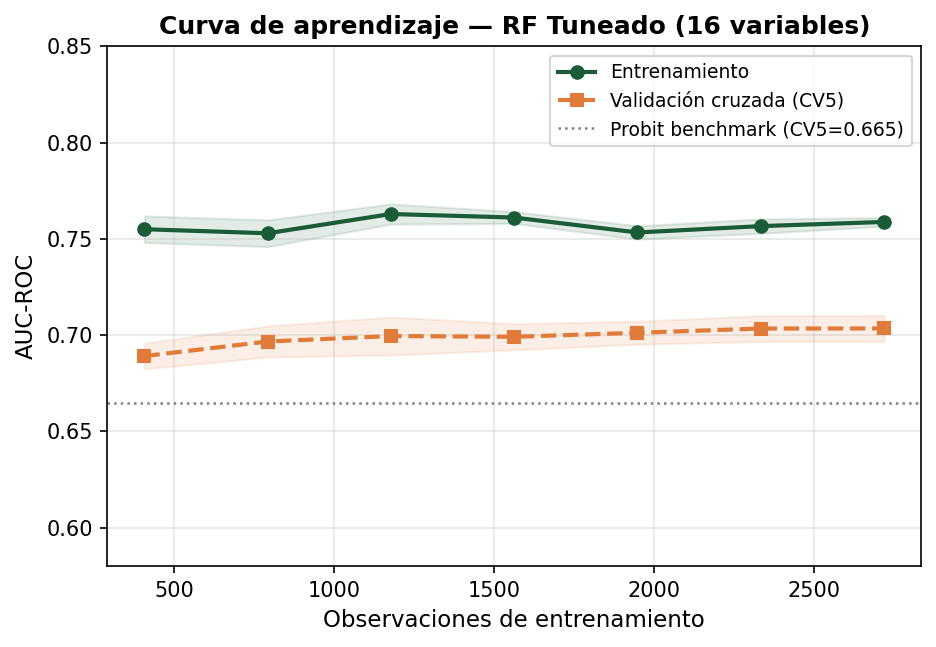
\includegraphics[width=0.82\textwidth]{../figures/curva_aprendizaje_rf.png}
\\
\vspace{0.15cm}
\scriptsize
Brecha \textit{train-CV5} estable en $\approx 0.057$ a lo largo del rango muestral.\\
Descarta memorización: el sobreajuste residual es el optimismo estructural del bagging sobre datos in-bag.\\
La curva de CV5 supera al benchmark Probit (línea punteada, 0.665) desde $n \approx 500$.
\end{frame}
